\begin{frame}{Controller design}{Optimal control}
	 \textbf{Definition of optimality}
	 \begin{itemize}
	 	\item Cost function
	 	\item Weighting of variables
	 	\item Horizons
	 	\item Constraints
	 	\item Benefits in comparison to pole-placement 
	 \end{itemize}
 
\begin{equation} \label{eq:lqr_cost_fcn}
	J = \int_0^{\infty} \left(x^TQx + u^TRu + 2x^TNu\right)dt
\end{equation}

\end{frame}

%%%%%%%%%%%%%%%%%%%%%%%%%%%%%%%%%%%%%%%%%%%%%%%%%%%

\begin{frame}{Controller design}{Linear Quadratic Regulator}
	 \textbf{Linear Quadratic Regulator}
	\begin{itemize}
		\item Cost function
		\item Infinite-horizon 
		\item Feedback law
		\item Drawbacks
	\end{itemize}

\begin{equation} \label{eq:lqr_cost_fcn}
	J = \int_0^{\infty} \left(x^TQx + u^TRu + 2x^TNu\right)dt
\end{equation}
\begin{equation} \label{eq:lqr_cost_fcn}
	u = -Kx
\end{equation}

\begin{equation} \label{eq:lqr_K}
	K = -R^{-1}B^{T}P
\end{equation}

where P is the unique solution to the algebraic Ricatti equation
\begin{equation} \label{eq:ricatti}
	A^TP + PA - PBR^{-1}B^TP+Q = 0
\end{equation}

\end{frame}


%%%%%%%%%%%%%%%%%%%%%%%%%%%%%%%%%%%%%%%%%%%%%%%%%%%

\begin{frame}{Controller design}{Linear Quadratic Regulator}
\begin{equation}
	Q =
	\left(\begin{array}{cccccccc}
		1 & 0 & 0 & 0 & 0 & 0 & 0 & 0  \\
		0 & 1 & 0 & 0 & 0 & 0 & 0 & 0  \\
		0 & 0 & 1 & 0 & 0 & 0 & 0 & 0  \\
		0 & 0 & 0 & 1 & 0 & 0 & 0 & 0  \\
		0 & 0 & 0 & 0 & 2 & 0 & 0 & 0  \\
		0 & 0 & 0 & 0 & 0 & 1 & 0 & 0  \\
		0 & 0 & 0 & 0 & 0 & 0 & 2 & 0  \\
		0 & 0 & 0 & 0 & 0 & 0 & 0 & 1
	\end{array}\right)
	\text{  and  }
	R =
	\left(\begin{array}{cc}
		1 & 0  \\
		0 & 0.025
	\end{array}\right)
\end{equation}

\medskip

\begin{equation}
	K =
	\left(\begin{array}{cccccccccc}
		-0.0784 &  -0.0140 &  -0.0203 &   1.1457 &  -0.1743 &  -0.1021 &  -0.6274 &   0.0049 \\
		0.5679 &   0.0786 &   0.1447 &  -4.0389 &   0.7489 &   0.4246 &   2.5119 &   0.0041
	\end{array}\right)
\end{equation}
	
\end{frame}

%%%%%%%%%%%%%%%%%%%%%%%%%%%%%%%%%%%%%%%%%%%%%%%%%%%%%%%%%%%%%%%%%%%%

\begin{frame}{Controller design}{Observer design}
	\textbf{Observer structure}
	\begin{itemize}
		\item Luenberger observer
		\item Separation Principle
		\item Observer pole placement
	\end{itemize}


\begin{equation} \label{eq:obs_error_dot}
	\dot{e} = (A - LC)e
\end{equation}
\begin{figure}[h!]
	\centering
	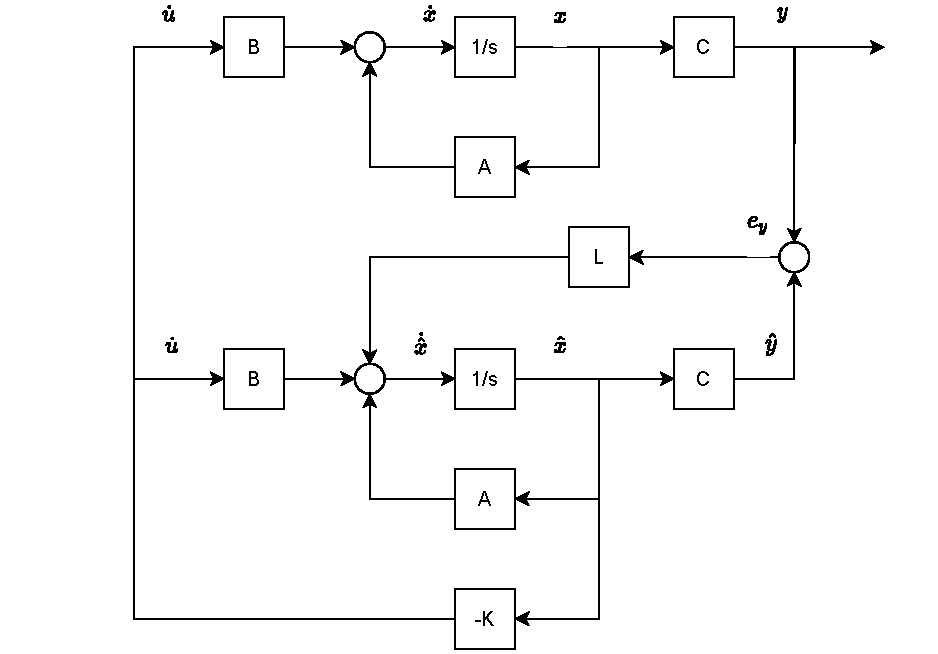
\includegraphics[width=0.5\textwidth]{../Graphics/Observer_diagram.pdf}
	\caption{Observer structure}
	\label{fig:obs_struct}
\end{figure}
\end{frame}




%%%%%%%%%%%%%%%%%